\documentclass[aspectratio=169,11pt]{beamer}
% docs/slides/preamble.tex -- 五份 deck 共享
\documentclass[aspectratio=169,11pt]{beamer}

% ==== 中文与字体 ====
\usepackage[UTF8,fontset=none]{ctex}
\usepackage{fontspec}

\IfFontExistsTF{PingFang SC}{%
  \setCJKmainfont{PingFang SC}[BoldFont=PingFang SC,ItalicFont=PingFang SC,AutoFakeSlant=0.15]
  \setCJKsansfont{PingFang SC}[ItalicFont=PingFang SC,AutoFakeSlant=0.15]
  \setCJKmonofont{PingFang SC}
}{%
  \IfFontExistsTF{Source Han Sans SC}{%
    \setCJKmainfont{Source Han Sans SC}
    \setCJKsansfont{Source Han Sans SC}
  }{%
    \IfFontExistsTF{Noto Sans CJK SC}{%
      \setCJKmainfont{Noto Sans CJK SC}
      \setCJKsansfont{Noto Sans CJK SC}
    }{%
      \setCJKmainfont{Heiti SC}
      \setCJKsansfont{Heiti SC}
    }
  }
}

\IfFontExistsTF{Helvetica Neue}{\setmainfont{Helvetica Neue}}{%
  \IfFontExistsTF{Inter}{\setmainfont{Inter}}{}}
\IfFontExistsTF{JetBrains Mono}{\setmonofont{JetBrains Mono}[Scale=0.85]}%
  {\setmonofont{Menlo}[Scale=0.85]}

% ==== 颜色 ====
\usepackage{xcolor}
\definecolor{cMain}{HTML}{1F4E79}
\definecolor{cAccent}{HTML}{E07A1F}
\definecolor{cGray}{HTML}{595959}
\definecolor{cMute}{HTML}{F4F4F4}
\definecolor{cOK}{HTML}{2E7D32}
\definecolor{cBad}{HTML}{B23A3A}
\definecolor{cWarn}{HTML}{C8A300}

% ==== 主题 ====
\usepackage{tcolorbox}
\usetheme{metropolis}
\metroset{progressbar=frametitle,numbering=fraction,block=fill}
\setbeamercolor{frametitle}{bg=cMain,fg=white}
\setbeamercolor{progress bar}{fg=cAccent,bg=cMute}
\setbeamercolor{alerted text}{fg=cAccent}
\setbeamercolor{title}{fg=cMain}

% metropolis 默认尝试 Fira Sans，未安装时 fallback 到 Latin Modern Sans。
% 这里在主题加载后显式覆盖，强制使用 macOS 上一定存在的 Helvetica Neue，
% 跟中文 PingFang 风格一致；找不到则按顺序尝试 Inter / Arial。
\IfFontExistsTF{Helvetica Neue}{%
  \setsansfont{Helvetica Neue}%
}{%
  \IfFontExistsTF{Inter}{\setsansfont{Inter}}{%
    \IfFontExistsTF{Arial}{\setsansfont{Arial}}{}}%
}

% ==== TikZ ====
\usepackage{tikz}
\usetikzlibrary{positioning,arrows.meta,fit,shapes.geometric,calc,%
  decorations.pathmorphing,backgrounds}

\tikzset{
  node-box/.style={draw=cMain,thick,rounded corners=2pt,
    minimum height=8mm,minimum width=18mm,align=center,font=\small},
  node-state/.style={draw=cMain,thick,circle,minimum size=14mm,
    align=center,font=\small},
  node-ok/.style={draw=cOK,thick,fill=cOK!10},
  node-warn/.style={draw=cWarn,thick,fill=cWarn!15},
  node-bad/.style={draw=cBad,thick,fill=cBad!10},
  % 色盲友好的状态机三态：蓝 (正常/Closed) / 橙 (告警/Open) / 灰 (中间/HalfOpen)
  % 避免 red-green 二元区分，改用 hue + lightness 双通道。
  node-state-normal/.style={draw=cMain,thick,fill=cMain!12},
  node-state-alert/.style={draw=cAccent,thick,fill=cAccent!18},
  node-state-transition/.style={draw=cGray,thick,fill=cGray!18},
  arrow/.style={-{Stealth[length=2mm]},thick,draw=cMain},
  arrow-async/.style={-{Stealth[length=2mm]},thick,dashed,draw=cGray},
  arrow-bad/.style={-{Stealth[length=2mm]},thick,draw=cBad},
  arrow-alert/.style={-{Stealth[length=2mm]},thick,draw=cAccent},
  lifeline/.style={dashed,thick,draw=cGray},
}

% ==== 代码 ====
\usepackage{listings}
\lstdefinelanguage{Go}{
  morekeywords={break,case,chan,const,continue,default,defer,else,
    fallthrough,for,func,go,goto,if,import,interface,map,package,range,
    return,select,struct,switch,type,var,nil,true,false,iota},
  morekeywords=[2]{string,int,int64,uint,uint64,bool,byte,error,context},
  sensitive=true,
  morecomment=[l]//,morecomment=[s]{/*}{*/},
  morestring=[b]",morestring=[b]`,
}
\lstdefinelanguage{LuaRedis}{
  morekeywords={and,break,do,else,elseif,end,false,for,function,if,in,
    local,nil,not,or,repeat,return,then,true,until,while},
  morekeywords=[2]{redis,call,KEYS,ARGV,tonumber,HGET,HSET,GET,SET,
    DECR,DECRBY,INCR,INCRBY,EXPIRE,PEXPIRE,ZADD,ZCARD,ZREMRANGEBYSCORE,
    EVAL,EVALSHA},
  sensitive=true,
  morecomment=[l]{--},
  morestring=[b]",morestring=[b]',
}

\lstdefinestyle{base}{
  basicstyle=\ttfamily\scriptsize,
  numbers=left,numberstyle=\tiny\color{cGray},
  keywordstyle=\color{cMain}\bfseries,
  keywordstyle=[2]\color{cAccent},
  stringstyle=\color{cOK},
  commentstyle=\color{cGray}\itshape,
  backgroundcolor=\color{cMute},
  frame=single,framerule=0pt,
  showstringspaces=false,
  breaklines=true,
  tabsize=2,
  columns=fullflexible,
}
\lstset{style=base}

% ==== 三线表与附录页码 ====
\usepackage{booktabs}
\usepackage{appendixnumberbeamer}

% ==== 页脚来源标注 ====
\newcommand{\srcnote}[1]{{\color{cGray}\scriptsize\itshape #1}}

% 关键论点框
\newcommand{\keypoint}[1]{%
  \begin{tcolorbox}[colback=cMute,colframe=cMain,boxrule=0.5pt,arc=2pt]%
  #1\end{tcolorbox}}

% 缩小本 deck 的代码字号，避免长 lstlisting 溢出
\lstset{basicstyle=\ttfamily\tiny}

\title{支付：钱即将出手的那一秒}
\subtitle{gomall /paydown 业务侧 deck —— 五角色视角看一次扣款}
\author{gomall · 业务侧 deck}
\date{}

\begin{document}

\maketitle

\begin{frame}[shrink]{今日大纲}
\tableofcontents
\end{frame}

% ============================================================
\section{业务定位：支付是 P0 中的 P0}
% ============================================================

\begin{frame}[shrink]{为什么单独拿一份 deck 讲支付}
\begin{itemize}
  \item 整个电商链路 20+ 环节，支付是\textbf{唯一让用户真正紧张的一秒}：钱即将离开账户。
  \item 浏览失败 = 再刷一次；下单失败 = 重填地址；支付失败 = 客诉、退款、平台兜底。
  \item gomall 的 SLO 里它属于 P0：\textbf{99.95\% 可用 / p99 < 500ms / 不挂限流}。
  \item 这意味着：每年最多宕 4 小时 22 分；用户排队也得放进来，不能 70001。
\end{itemize}
\keypoint{支付不是"一个接口"，而是"商业信任的具体落点"。每一行代码背后都有一条客诉路径。}
\srcnote{README.md 业务承诺表；internal/payment/routes.go:14--21 paydown 中间件栈}
\end{frame}

\begin{frame}[shrink]{五角色眼中的同一秒}
\small
\begin{tabular}{@{}lp{8.5cm}@{}}
\toprule
角色 & 那一秒最焦虑的事 \\
\midrule
C 端用户 & "我的钱扣了吗 / 订单成了吗 / 重复扣了怎么办" \\
商家 & "什么时候到账 / 平台抽多少 / 退款会不会扣回去" \\
运营 & "GMV 落账瞬间能不能扛峰 / 这分钟卡了多少订单" \\
客服 & "扣款没出货 / 支付后掉单 / 重复扣款"三大客诉 \\
SRE & "p99 还在 500ms 以内吗 / 第三方挂了会不会全站陪葬" \\
\bottomrule
\end{tabular}
\vspace{2mm}
\begin{itemize}\small
  \item 本 deck 后续每一帧都标注\textbf{它在回答哪个角色的哪个问题}。
  \item 业务码 60002 / 70002 / 30001 都会出现在客服话术里。
\end{itemize}
\srcnote{README.md 业务全景表；pkg/e/code.go:53--58}
\end{frame}

\begin{frame}[shrink]{业务后果数字化}
\begin{itemize}
  \item 支付掉单率每升 \textbf{1 pp}：按 GMV 1000 万/日估算 = 单日 \textbf{10 万元} 直接流失；二次复购率再掉 0.5 pp。
  \item 客诉一通电话客服平均 \textbf{8 分钟}：日 1000 单掉单 $\to$ 客服需 \textbf{2.2 个人日} 兜底。
  \item 第三方支付 30s 超时不熔断：用户白屏放弃下单率 \textbf{~38\%}（行业经验）。
  \item 熔断打开期间损失 5\% 用户 vs 不熔断雪崩全站损失 100\%：\textbf{两个数量级}差。
\end{itemize}
\keypoint{所有看起来"过度设计"的中间件，背后都是一条算得出钱的客诉路径。}
\srcnote{stressTest/REPORT.md §1 链路压测；internal/payment/routes.go:14--21}
\end{frame}

\begin{frame}[shrink]{/paydown 在 gomall 业务全景中的位置}
\begin{tikzpicture}[node distance=6mm and 10mm]
  \node[node-box] (cart)  {加购选地址\\deck 04};
  \node[node-box,right=of cart] (order) {下单锁库存\\deck 04+07};
  \node[node-box,right=of order,node-warn] (pay)   {\textbf{支付}\\本 deck};
  \node[node-box,right=of pay] (ship)  {商家发货\\deck 09};
  \node[node-box,below=of pay,node-bad]  (refund){退款 / 售后\\deck 09};
  \draw[arrow] (cart)  -- (order);
  \draw[arrow] (order) -- (pay);
  \draw[arrow] (pay)   -- (ship);
  \draw[arrow-bad] (pay) -- (refund);
\end{tikzpicture}
\vspace{1mm}
\begin{itemize}\small
  \item 上游：下单已经把库存预占进 Redis \texttt{reserved} 桶。
  \item 下游：支付成功 $\to$ outbox 事件 \texttt{order.paid} $\to$ 通知发货 / 优惠券核销 / 索引更新。
  \item 失败兜底：30 分钟未付 $\to$ Cron + RMQ 双保险关单（deck 09）。
\end{itemize}
\srcnote{internal/payment/routes.go:14--21；internal/order/cancel.go}
\end{frame}

\begin{frame}[shrink]{业务边界：本支付\textbf{不做}什么}
\begin{itemize}
  \item \textbf{不真接支付宝 / 微信 / 银联}：README 已经写了 —— "法币支付走 outbox 事件，下游对接由 wallet 服务消费（路线图）"。
  \item \textbf{不做实名 KYC}：合规上属银行 + 持牌支付公司的事。
  \item \textbf{不做风控引擎}：异常交易识别 / 黑名单 / 行为模型留给独立风控团队。
  \item \textbf{不做反洗钱（AML）}：上链 / 大额拆分识别走独立合规系统。
  \item \textbf{不做商家分账}：平台抽成 / 服务费 / 代收代付路线图。
  \item \textbf{不做发票管理}：增值税专票 / 普票留给财税系统。
\end{itemize}
\keypoint{诚实划边界 = 给商家和合规一个交代。MVP 阶段聚焦"扣款 + 入账 + 状态机推进"三件事做到位。}
\srcnote{README.md §业务边界（不做什么）}
\end{frame}

\begin{frame}[shrink]{业务边界图：本 deck 在哪里、不在哪里}
\begin{tikzpicture}[node distance=5mm and 8mm]
  \node[node-box,node-ok]   (in1) {扣买家余额};
  \node[node-box,node-ok,right=of in1] (in2) {入卖家余额};
  \node[node-box,node-ok,right=of in2] (in3) {订单状态推进};
  \node[node-box,node-ok,right=of in3] (in4) {outbox 通知下游};
  \node[node-box,node-bad,below=of in1] (out1) {真实第三方网关};
  \node[node-box,node-bad,right=of out1] (out2) {KYC / 风控 / AML};
  \node[node-box,node-bad,right=of out2] (out3) {商家分账};
  \node[node-box,node-bad,right=of out3] (out4) {发票 / 财税};
\end{tikzpicture}
\vspace{1mm}
\small 上排（绿）= 本 deck 必须做对；下排（红）= 路线图，不在本 deck 范围。但 \textbf{paydown 接口已为真接第三方留好位置}（熔断器已挂、outbox 已通），见 §3。
\srcnote{README.md §业务边界；internal/payment/routes.go:14--21}
\end{frame}

% ============================================================
\section{合规与信任：为什么金额要加密}
% ============================================================

\begin{frame}[shrink]{客服 / 法务的视角：明文金额会出什么事}
\begin{itemize}
  \item \textbf{客服}：用户来电"我的余额怎么少了 50 块"。如果 DBA 能直查 \texttt{users.money}，举证就停在"我说没动你也没法证明"。
  \item \textbf{法务}：等保 2.0 / GB/T 22239 / PCI-DSS 要求"敏感金额字段不得明文落盘"，年审过不了 = 不能上线大促。
  \item \textbf{运营}：拖库新闻一旦上热搜（明文金额泄漏），日均订单跌 \textbf{30--50\%}（行业事件经验）。
  \item \textbf{内控}：明文金额一旦被 \texttt{log.Debug(user)} 序列化 $\to$ 上传 ELK $\to$ 全公司有 ELK 账号的人都能看。
\end{itemize}
\keypoint{加密金额不是"加密功能"，是\textbf{把金额从数据库视野里抹掉}。运维 / DBA / 实习生看到的永远是乱码。}
\srcnote{internal/user/model.go:64--101}
\end{frame}

\begin{frame}[shrink]{AES 金额加密的合规业务价值（不只是技术）}
\begin{itemize}
  \item \textbf{合规审计}：年审看的是"敏感字段是否加密 + 密钥是否分离 + 是否能审计明文访问路径"。三条都满足，过审周期从 6 周缩到 2 周。
  \item \textbf{商家结算单脱敏}：商家后台看到的金额是 \textbf{明文（业务必须）}，但需要客服 / 平台审计能力时，DB 直查永远只能拿到密文 —— 一次明文访问必须走 \texttt{DecryptMoney} 函数 $\to$ 可被审计日志覆盖。
  \item \textbf{财务对账}：财务看的是脱敏后的聚合报表（GMV / 商户日入），由结算服务定时拉取后\textbf{一次性解密入数仓}，DB 永远不存明文。
  \item \textbf{业务取舍代价}：\texttt{SUM(money)} 在 DB 里\textbf{无法直接聚合}（密文异序）—— 财务报表必须走结算服务批跑，不能裸 SQL。
\end{itemize}
\srcnote{internal/user/model.go:64--101；pkg/utils/encryption/money\_encrypt.go}
\end{frame}

\begin{frame}[shrink]{gomall 的金额加密链路}
\begin{tikzpicture}[node distance=8mm and 14mm]
  \node[node-box] (u) {Client\\req.Key};
  \node[node-box,right=of u] (svc) {PayDown};
  \node[node-box,right=of svc,node-warn] (aes) {AES-128-CBC\\(MoneySecret + key)};
  \node[node-box,below=of aes] (db) {MySQL users.money\\密文};
  \draw[arrow] (u) -- node[above,font=\tiny]{支付密码} (svc);
  \draw[arrow] (svc) -- node[above,font=\tiny]{加/解密} (aes);
  \draw[arrow] (aes) -- node[right,font=\tiny]{读写} (db);
\end{tikzpicture}
\vspace{1mm}
\begin{itemize}
  \item 双密钥：服务端 \texttt{MoneySecret} + 用户支付密码 \texttt{key}。
  \item 任一方泄漏\textbf{都不足以}独立解密 $\to$ 密钥分离。
  \item 改密码 = 解密旧密文 + 用新 key 重新加密。
\end{itemize}
\srcnote{internal/user/model.go:64--101；config/locales/config.yaml.example 中 MoneySecret 字段}
\end{frame}

\begin{frame}[fragile,shrink]{加解密的代码长这样}
\begin{lstlisting}[language=Go,firstnumber=64,
  caption={\srcnote{internal/user/model.go:64--101 节选}}]
// EncryptMoney 加密金额。底层库加密失败 panic，统一折叠为 error
func (u *User) EncryptMoney(key string) (money string, err error) {
    defer func() { if r := recover(); r != nil {
        money, err = "", errors.New("余额加密失败") } }()
    aesObj, err := secret.NewAesEncrypt(
        conf.Config.EncryptSecret.MoneySecret, // 服务端持有
        key,                                   // 用户支付密码
        "", secret.AesEncrypt128, secret.AesModeTypeCBC)
    if err != nil { return }
    money = aesObj.SecretEncrypt(u.Money)
    return
}

// DecryptMoney 解密金额，返回值单位为分
func (u *User) DecryptMoney(key string) (money int64, err error) {
    defer func() { if r := recover(); r != nil {
        money, err = 0, ErrMoneyKeyIncorrect } }() // 错密钥去填充越界
    aesObj, err := secret.NewAesEncrypt(
        conf.Config.EncryptSecret.MoneySecret, key, "",
        secret.AesEncrypt128, secret.AesModeTypeCBC)
    if err != nil { return }
    plain := aesObj.SecretDecrypt(u.Money)
    money, err = strconv.ParseInt(plain, 10, 64)
    if err != nil { return 0, ErrMoneyKeyIncorrect } // 乱码不当余额
    return money, nil
}
\end{lstlisting}
\end{frame}

\begin{frame}[shrink]{逐行讲解：加解密对业务承诺的兑现点}
\begin{itemize}\small
  \item \textbf{71/90 行 服务端密钥 + 用户密码独立}：DBA 拿走 dump 也无能为力（缺密码）；用户密码被钓鱼也只能搞一个账号（缺服务端密钥）。两道防线分别给法务和反钓鱼。
  \item \textbf{71/90 行 CBC 而非 ECB}：同一笔金额每次密文不同 —— 防"对照表猜金额"，对应风控诉求。
  \item \textbf{model.go:27 \texttt{Money string}}：密文长度可变。代价 = SQL 直接 \texttt{SUM} / \texttt{ORDER BY money} 行不通，必须走结算服务（业务取舍）。
  \item \textbf{96 行 \texttt{strconv.ParseInt}}：单位是\textbf{分} —— 全链路避免浮点，对应"100 元订单分账误差 0.01 元"客诉。
  \item \textbf{错误传播}：密码错 $\to$ CBC 去填充 panic 或解出乱码 $\to$ \texttt{recover}/\texttt{ParseInt} 统一折叠为 \texttt{ErrMoneyKeyIncorrect} $\to$ TX 回滚。早期实现里这条路径会把整个请求 panic 掉，现在是明确的"支付密码错误"业务错误。
\end{itemize}
\srcnote{internal/user/model.go:80--101 DecryptMoney；:15--16 ErrMoneyKeyIncorrect}
\end{frame}

\begin{frame}[shrink]{业务取舍：金额加密对 SQL 聚合的代价}
\small
\begin{tabular}{@{}lll@{}}
\toprule
查询场景 & 明文方案 & 密文方案 \\
\midrule
"商家日入" & \texttt{SUM(money) GROUP BY boss\_id} 秒级 & 结算服务批跑 + 缓存 \\
"用户余额排行" & \texttt{ORDER BY money} 秒级 & 不支持，业务侧改埋点 \\
"对账" & SQL 比对 & 解密后入数仓 \\
\bottomrule
\end{tabular}
\vspace{2mm}
\begin{itemize}\small
  \item 代价是\textbf{放弃 DB 侧大数据聚合能力}。
  \item 收益是\textbf{合规通过 + 拖库零金额泄漏}。
  \item 业务侧的选择：交易类金额\textbf{必须密文}（盘比合规重要），统计类指标走数仓 / 缓存（精度可后补）。
\end{itemize}
\srcnote{internal/user/model.go:64--101}
\end{frame}

% ============================================================
\section{支付密码：业务侧二次验证的取舍}
% ============================================================

\begin{frame}[shrink]{为什么不直接用"实名 + 短信验证码"}
\begin{itemize}
  \item \textbf{实名 KYC 的合规成本}：要接公安一二三要素接口（人均 0.5--2 元 / 次），运营商短信通道（0.05 元 / 条），并备案"信息处理者"身份 $\to$ \textbf{合规审批 6+ 月}。
  \item \textbf{业务收益对照}：电商扣款金额一般 < 1000 元 / 笔，风险敞口与全链 KYC 不匹配。
  \item \textbf{客诉路径}：短信验证码到达率 \textbf{96--98\%} $\to$ 每天 \textbf{2--4\%} 用户因收不到验证码放弃支付。
  \item \textbf{业务侧的选择}：用\textbf{业务侧 6 位支付密码} —— 不存盘、入口校验、AES 入参，覆盖 95\% 场景；KYC + 短信留给"大额提现 / Web3 / 银行卡绑定"路线图。
\end{itemize}
\srcnote{internal/payment/service.go:43--47；consts/user.go:35 EncryptMoneyKeyLength}
\end{frame}

\begin{frame}[shrink]{支付密码 vs 登录密码：业务上为什么分两套}
\small
\begin{tabular}{@{}lll@{}}
\toprule
        & 登录密码     & 支付密码     \\
\midrule
作用    & 拿 JWT      & 解密金额     \\
长度    & $\geq 6$    & 固定 6 位    \\
泄漏后果 & 看订单地址  & 直接扣款     \\
存储    & bcrypt 哈希 & \textbf{不存}    \\
重置    & 邮箱 + 短信 & 客服核身 + 余额冻结 \\
客服话术 & "已发重置链接" & "请验证身份后由客服重置，48h 内余额冻结" \\
\bottomrule
\end{tabular}
\vspace{1mm}
\begin{itemize}\small
  \item 支付密码\textbf{不存}：用户每次手输 $\to$ 整库 dump 也解不开。
  \item 入口校验 \texttt{len(req.Key) == 6}，太短直接拒（防 SQL 注入测试 / 弱口令撞库）。
  \item 客服只能"冻结余额 48h + 用户本人重置后解冻"，不可代输支付密码。
\end{itemize}
\srcnote{internal/payment/service.go:43--47；consts/user.go:35}
\end{frame}

\begin{frame}[shrink]{支付密码弱口令的客诉路径}
\resizebox{0.95\textwidth}{!}{%
\begin{tikzpicture}[node distance=8mm and 16mm,font=\scriptsize]
  \node[node-box] (u) {用户支付};
  \node[node-box,right=of u,node-warn] (a) {6 位短密码\\被穷举};
  \node[node-box,right=of a,node-bad] (b) {账户余额\\被盗刷};
  \node[node-box,below=of b] (c) {客诉电话};
  \node[node-box,left=of c] (d) {客服核身\\冻结余额};
  \node[node-box,left=of d] (e) {审计日志\\追加密访问};
  \draw[arrow] (u) -- (a);
  \draw[arrow-bad] (a) -- (b);
  \draw[arrow] (b) -- (c);
  \draw[arrow] (c) -- (d);
  \draw[arrow] (d) -- (e);
\end{tikzpicture}}
\vspace{1mm}
\begin{itemize}\small
  \item 弱口令风险敞口：6 位 = 100 万组合，单接口 5 RPS 也能穷举完一天。
  \item \textbf{为何还能用}：因为接口前面挂了 \textbf{CircuitBreaker + RateLimit + Idempotency} 三层，单 IP 单用户实际穷举速率 < 0.5 RPS $\to$ 跑完平均 \textbf{23 天}，余额早被风控冻结。
  \item 路线图：路线图阶段对\textbf{风控引擎}（异地 IP / 行为模型）做对接。
\end{itemize}
\srcnote{middleware/ratelimit.go；middleware/circuitbreaker.go；internal/payment/service.go:43--47}
\end{frame}

% ============================================================
\section{PayDown 主体：一次扣款里的五件业务事}
% ============================================================

\begin{frame}[shrink]{业务侧的四个硬约束}
\begin{tabular}{@{}lll@{}}
\toprule
约束 & 业务诉求 & 设计回应 \\
\midrule
金额不能明文落盘 & 合规 / 防内鬼 / 防误日志 & AES-128-CBC + 双密钥 \\
密码错不能扣款 & 防穷举 / 防钓鱼 & 长度校验 + 解密失败 abort \\
第三方支付会挂 & 不让 5\% 拖垮 100\% & CircuitBreaker 5/10s/3 \\
客户端会重试 & "重复扣款"是 top1 客诉 & Idempotency-Key + Lua \\
\bottomrule
\end{tabular}
\vspace{2mm}
\small 四条由\textbf{合规 + 客诉 + 监控}三方倒推。\textbf{业务码地图}：30001 token 错 / 60002 处理中 / 70001 限流 / 70002 熔断。
\srcnote{internal/payment/routes.go:14--21 paydown 完整中间件栈；pkg/e/code.go:53--58}
\end{frame}

\begin{frame}[shrink]{PayDown 在一次事务里做的几件事}
\begin{tikzpicture}[node distance=5mm and 7mm,font=\small]
  \node[node-box] (s1) {1.取订单\\(UnPaid?)};
  \node[node-box,right=of s1] (s2) {2.扣买家\\+debit 流水};
  \node[node-box,right=of s2] (s3) {3.入卖家\\+credit 流水};
  \node[node-box,below=of s2] (s4) {4.减库存\\+翻状态};
  \node[node-box,right=of s4] (s5) {5.写 outbox\\order.paid};
  \node[node-box,below=of s5,node-bad] (rb) {任一失败\\TX rollback};
  \draw[arrow] (s1) -- (s2);
  \draw[arrow] (s2) -- (s3);
  \draw[arrow] (s3) |- (s4);
  \draw[arrow] (s4) -- (s5);
  \draw[arrow-bad] (s5) -- (rb);
\end{tikzpicture}
\vspace{1mm}
\small 全部落在同一 \texttt{tx}，\textbf{要么全成功要么全不动}。扣买家 / 入卖家\textbf{各自带一条不可变流水}（debit / credit，§4），余额变动与流水同生共死；outbox 也在 TX 内写 —— 事务消息防丢（deck 11 主题）。\textbf{业务承诺}：客户端拿到 200 status=200 即代表"钱扣了 / 商家入账了 / 两条流水落账 / 库存减了 / 下游必定收到事件"都已落定。
\srcnote{internal/payment/service.go:55--218}
\end{frame}

\begin{frame}[shrink]{PayDown 结算的标准时序：六方一次扣款}
\centering
\resizebox{0.92\textwidth}{!}{%
\begin{sequencediagram}
  \newthread{u}{用户}
  \newinst[1]{h}{Payment Handler}
  \newinst[1]{d}{订单/用户 DAO}
  \newinst[1]{l}{台账 money}
  \newinst[1]{o}{Outbox}
  \newinst[1]{q}{RabbitMQ}

  \begin{call}{u}{POST /paydown (支付密码)}{h}{200 OK}
    \begin{call}{h}{开事务 · 锁买卖双方 FOR UPDATE}{d}{校验支付密码 OK}
    \end{call}
    \begin{call}{h}{买家扣款 / 卖家入账 (折后实付 FinalCents)}{d}{余额密文回写}
    \end{call}
    \begin{call}{h}{追加 debit + credit 复式记账流水}{l}{同事务落账}
    \end{call}
    \begin{call}{h}{DeductStock 扣库存 · MarkOrderPaid (WaitPay 守卫)}{d}{状态推进}
    \end{call}
    \begin{call}{h}{写 order.paid 事件}{o}{同事务 commit}
    \end{call}
  \end{call}

  \mess{o}{异步投递 OrderPaid}{q}
\end{sequencediagram}}

\vspace{1mm}
\small 扣款、入账、台账流水、库存、改单、发件箱六件事落在\textbf{同一个事务}里，要么全成功要么全回滚。用户拿到 \texttt{200 OK} 即代表六者皆已落定；\texttt{order.paid} 事件由 Outbox 发布器\textbf{事务外异步}投递给 RabbitMQ，下游发货 / 核销 / 索引各自消费。
\srcnote{internal/payment/service.go:55--218 PayDown 事务体；:208--218 outbox.Insert}
\end{frame}

\begin{frame}[fragile,shrink]{PayDown 扣款这一段的真实代码}
\begin{lstlisting}[language=Go,firstnumber=79,
  caption={\srcnote{internal/payment/service.go:79--114 节选}}]
// 实付口径：命中满减以折后实付 FinalCents 为准，否则单价 * 件数
payable := order.Money * int64(num)
if order.PromoRuleID != 0 {            // 用命中标识判据，不用 FinalCents>0
    payable = order.FinalCents         // 立减到 0 也是合法实付
}

buyer, err := userDao.GetUserByIdForUpdate(uId)  // 行锁，杜绝并发双扣
if err != nil { return err }
if !buyer.CheckMoneyPassword(req.Key) {          // 密码与余额解密分离
    return user.ErrMoneyKeyIncorrect
}
userMoney, err := buyer.DecryptMoney()
if err != nil { return err }
if userMoney-payable < 0 { return errors.New("金额不足") } // TX 内回滚

buyerBalanceAfter := userMoney - payable
buyer.Money = strconv.FormatInt(buyerBalanceAfter, 10)
buyer.Money, err = buyer.EncryptMoney()          // 重新加密落库
if err != nil { return err }
err = userDao.UpdateUserById(uId, buyer)
\end{lstlisting}
\end{frame}

\begin{frame}[shrink]{逐行讲解：扣款这一步的业务含义}
\begin{itemize}\small
  \item \textbf{64 行 OrderWaitPay 校验在 TX 内}：不能 TX 外读再进事务 —— 否则典型 TOCTOU，两并发支付都看到待付款 $\to$ 双扣。这是"重复扣款"客诉的根因之一。
  \item \textbf{79--82 行 实付口径}：命中满减时 \texttt{payable} 取折后实付 \texttt{FinalCents}，否则单价 $\times$ 件数兜底。判据用 \texttt{PromoRuleID != 0} 而\textbf{不是} \texttt{FinalCents > 0} —— 满减立减到 0 / 100\% 折扣时 \texttt{FinalCents == 0} 是合法实付，用大于零误判为未命中会回退全价多扣买家。
  \item \textbf{86 行 \texttt{GetUserByIdForUpdate}}：行锁读买家，把"读余额 $\to$ 判断 $\to$ 改写"串行化，并发两笔支付不会都拿到旧余额。
  \item \textbf{91 行 \texttt{CheckMoneyPassword}}：支付密码校验与余额 AES 解密\textbf{分离}，密码错 $\to$ \texttt{ErrMoneyKeyIncorrect} $\to$ TX 回滚；穷举防护交给前置限流 + 熔断 + 幂等三层。
  \item \textbf{金额不足也 \texttt{return err}}：让 TX 走 rollback，\texttt{order.Type} 不推进，客户端可原 OrderId 充值后重试 —— 客服话术："充值后原订单可直接付款，30 分钟内有效"。
\end{itemize}
\srcnote{internal/payment/service.go:79--114；internal/user/model.go:15--16 ErrMoneyKeyIncorrect}
\end{frame}

\begin{frame}[fragile,shrink]{outbox 写在事务尾 —— 业务承诺的兑现点}
\begin{lstlisting}[language=Go,firstnumber=208,
  caption={\srcnote{internal/payment/service.go:208--218}}]
// outbox 事件：order.paid，投递交给 publisher 异步
return outbox.NewOutboxDaoByDB(tx).Insert(
    "order", "OrderPaid", "order.paid", order.ID,
    events.OrderPaid{
        OrderID: order.ID, OrderNum: order.OrderNum,
        UserID: uId, ProductID: productID, Num: num,
    },
)
\end{lstlisting}
\vspace{1mm}
\small \texttt{outbox.Insert} 用\textbf{同一个 tx} —— 事务消息：扣款与"已发事件"同生共死，\textbf{绝不会"钱扣了但下游没收到"}。Redis 预占释放走 TX 外，失败仅记日志，对账兜底。\textbf{业务下游}：发货通知 / 优惠券核销 / ES 索引更新 / 商家看板更新 / 财务对账增量。
\srcnote{internal/payment/service.go:228 cache.CommitReservation；deck 11 outbox 主题}
\end{frame}

\begin{frame}[shrink]{客服 SOP：用户报"扣款没出货"怎么查}
\begin{tikzpicture}[node distance=5mm and 8mm]
  \node[node-box] (q) {用户报\\"扣了没货"};
  \node[node-box,right=of q] (a) {查订单\\type 字段};
  \node[node-box,right=of a] (b) {查 outbox\\order.paid};
  \node[node-box,below=of b] (c) {查 RMQ\\消费者日志};
  \node[node-box,left=of c] (d) {查 Redis\\reserved};
  \node[node-box,left=of d] (e) {结论\\+ 处理};
  \draw[arrow] (q) -- (a);
  \draw[arrow] (a) -- (b);
  \draw[arrow] (b) -- (c);
  \draw[arrow] (c) -- (d);
  \draw[arrow] (d) -- (e);
\end{tikzpicture}
\vspace{1mm}
\small
\begin{tabular}{@{}lll@{}}
\toprule
情况 & 表征 & 客服动作 \\
\midrule
TX 失败回滚 & order=UnPaid + 余额未减 & 让用户重试，无影响 \\
扣了但 outbox 未发 & order=Paid + outbox 无行 & \textbf{不可能}，TX 原子 \\
outbox 已发未消费 & outbox pending > 5min & 提工单升级 SRE \\
消费失败 & outbox dead & 人工补发 \\
\bottomrule
\end{tabular}
\srcnote{internal/payment/service.go:208--218；internal/shared/outbox/repo.go}
\end{frame}

% ============================================================
\section{资金台账：复式记账补上"不可对账"硬伤}
% ============================================================

\begin{frame}[shrink]{业务困局：余额是一个密文列，扣款不留痕}
\begin{itemize}
  \item 早先钱包余额就是 \texttt{users.money} 上一个 AES 密文列：扣买家 = 改这个列，入卖家 = 改那个列，\textbf{改完什么都不留}。
  \item \textbf{财务}："这个月平台少了 3000 块，是哪几笔、谁扣的、扣给了谁？" —— 没流水，查不出来，只能认账。
  \item \textbf{客服}：用户报"我余额莫名少了 50"，DB 只能看到当前一个密文数，\textbf{看不到这 50 是哪一单扣的}，无从举证。
  \item \textbf{审计 / 风控}：资损发生后想回放"这笔钱怎么走的"，没有任何事件序列可重放。
  \item \textbf{对账}：账户余额与订单流水对不上时，没有第三本账做交叉验证 —— 一旦某次扣款代码有 bug 多扣 / 漏入，永远发现不了。
\end{itemize}
\keypoint{"余额是一个会被覆盖的数字"是支付系统的硬伤。真正的钱包系统，余额必须是\textbf{流水累加出来的结果}，而不是一个可以随手改的列。}
\srcnote{internal/payment/service.go:106--157 余额读改写；internal/money/ledger\_model.go:18--26}
\end{frame}

\begin{frame}[shrink]{解法：复式记账（debit / credit）流水台账}
\begin{itemize}\small
  \item 借鉴会计的\textbf{复式记账}：任何一笔资金转移都\textbf{成对记两条}——一方借记（debit，余额减少），一方贷记（credit，余额增加），两条金额相等、方向相反。
  \item 一次支付 100 元 $\to$ 买家记一条 debit 100、卖家记一条 credit 100。\textbf{全表 SUM(debit) 应恒等于 SUM(credit)}，这就是对账的数学保证（资金守恒）。
  \item 新增 \texttt{account\_transaction} 表，每条流水\textbf{不可变}（append-only，只插不改不删）：\texttt{user\_id / direction / amount\_cents / ref\_order\_id / balance\_after\_cents / biz\_type / created\_at}。
  \item 关键：\texttt{amount\_cents} 与 \texttt{balance\_after\_cents} 都是\textbf{明文 int64 分}，\textbf{不加密} —— 流水台账就是给对账 / 审计用的，必须能 \texttt{SUM} / \texttt{GROUP BY}。
  \item 与 \texttt{users.money} 的取舍刚好相反：余额密文（防拖库泄漏），流水明文（要对账）。两本账各司其职。
\end{itemize}
\srcnote{internal/money/ledger\_model.go:7--36；internal/migrate/migrate.go:44 注册 AutoMigrate}
\end{frame}

\begin{frame}[fragile,shrink]{表结构：account\_transaction}
\begin{lstlisting}[language=Go,firstnumber=7,
  caption={\srcnote{internal/money/ledger\_model.go:7--36}}]
const (                              // 复式记账两个方向
    DirectionDebit  = "debit"        // 借记：账户余额减少
    DirectionCredit = "credit"       // 贷记：账户余额增加
)
const BizTypeOrderPay = "order_pay"  // 流水来源，对账时区分

type AccountTransaction struct {
    dbmodel.Model
    UserID    uint   `gorm:"index:idx_acct_tx_user"`
    Direction string `gorm:"size:8;uniqueIndex:uniq_acct_tx_order_dir,priority:2"`
    AmountCents       int64  // 明文分，绝不加密
    RefOrderID        uint   `gorm:"uniqueIndex:uniq_acct_tx_order_dir,priority:1"`
    BalanceAfterCents int64  // 本次变更后余额，可回放
    BizType           string `gorm:"size:32"`
}
func (AccountTransaction) TableName() string { return "account_transaction" }
\end{lstlisting}
\vspace{1mm}
\small \texttt{(ref\_order\_id, direction)} 联合\textbf{唯一索引}是幂等的兜底：同一订单同一方向只可能插一条，重复入账撞唯一冲突直接报错回滚。\texttt{balance\_after\_cents} 记下每次变更后的余额快照 $\to$ 哪怕密文余额列被改坏，也能用流水\textbf{逐条回放重建}出正确余额。
\end{frame}

\begin{frame}[shrink]{一次支付的双写：余额列 + 流水台账（同事务）}
\begin{tikzpicture}[node distance=5mm and 8mm,font=\scriptsize]
  \node[node-box,node-warn] (tx) {PayDown 同一 tx};
  \node[node-box,node-ok,below left=6mm and 3mm of tx] (bm) {users.money\\买家密文 -100};
  \node[node-box,node-ok,below right=6mm and 3mm of tx] (sm) {users.money\\卖家密文 +100};
  \node[node-box,below=9mm of bm] (bl) {account\_transaction\\debit 100 / order=N};
  \node[node-box,below=9mm of sm] (sl) {account\_transaction\\credit 100 / order=N};
  \draw[arrow] (tx) -- (bm);
  \draw[arrow] (tx) -- (sm);
  \draw[arrow] (bm) -- node[left,font=\tiny]{追加流水} (bl);
  \draw[arrow] (sm) -- node[right,font=\tiny]{追加流水} (sl);
  \draw[arrow-bad,dashed] (bl) to[bend right=18] node[below,font=\tiny]{任一失败全回滚} (sl);
\end{tikzpicture}
\vspace{0.5mm}
\scriptsize 四个写（两个余额列 + 两条流水）落在\textbf{同一个事务}：要么 100 元从买家流到卖家且两条流水都在，要么什么都没发生。\textbf{绝不会出现"余额改了但没流水"或"流水有了但余额没动"}—— 这正是早先单写余额列做不到的对账闭环。
\srcnote{internal/payment/service.go:120--157 同事务两次 AppendTransaction}
\end{frame}

\begin{frame}[fragile,shrink]{PayDown 同事务追加 debit / credit 两条流水}
\begin{lstlisting}[language=Go,firstnumber=120,
  caption={\srcnote{internal/payment/service.go:120--157 节选}}]
// 买家扣款流水：与余额变动同事务追加
ledgerDao := money.NewLedgerDaoByDB(tx)          // 接管调用方的 tx
if err = ledgerDao.AppendTransaction(uId, order.ID,
    money.DirectionDebit, payable, buyerBalanceAfter,
    money.BizTypeOrderPay); err != nil { return err }
// ... 卖家余额读改写：bossBalanceAfter = bossMoney + payable ...
// 卖家入账流水：方向与买家相反，同一 order.ID
if err = ledgerDao.AppendTransaction(bossID, order.ID,
    money.DirectionCredit, payable, bossBalanceAfter,
    money.BizTypeOrderPay); err != nil { return err }
\end{lstlisting}
\begin{lstlisting}[language=Go,firstnumber=20,
  caption={\srcnote{internal/money/ledger\_repo.go:20--38}}]
// NewLedgerDaoByDB 接管调用方 tx，流水写入与余额变动同一原子提交
func NewLedgerDaoByDB(db *gorm.DB) *LedgerDao { return &LedgerDao{db} }
func (d *LedgerDao) AppendTransaction(userID, refOrderID uint,
    direction string, amountCents, balanceAfterCents int64,
    bizType string) error { /* Create(&AccountTransaction{...}) */ }
\end{lstlisting}
\end{frame}

\begin{frame}[shrink]{逐行讲解：流水追加的业务含义}
\begin{itemize}\small
  \item \textbf{121 行 \texttt{NewLedgerDaoByDB(tx)}}：\textbf{接管} PayDown 传进来的同一个 \texttt{tx}，而不是新开连接。这是"流水与余额同生共死"的命门 —— 余额改了流水必在，流水写失败余额改动一起回滚。
  \item \textbf{122 行 买家 debit}：\texttt{payable}（折后实付）作为金额，\texttt{buyerBalanceAfter} 是\textbf{扣款后}的余额快照，方向 \texttt{debit}。
  \item \textbf{154 行 卖家 credit}：同一个 \texttt{order.ID}，金额相同，方向\textbf{相反}，\texttt{bossBalanceAfter} 是\textbf{入账后}余额。一借一贷成对出现 $\to$ 资金守恒。
  \item \textbf{两条都用 \texttt{payable}}：流水金额与实际余额变动\textbf{同口径}（都是折后实付），绝不会出现"流水记全价、余额扣折后价"的对账裂缝。
  \item \textbf{失败即回滚}：\texttt{AppendTransaction} 返回 error 直接 \texttt{return} $\to$ 整个 PayDown 事务回滚，余额、库存、订单状态、outbox 全部不落地。
\end{itemize}
\srcnote{internal/payment/service.go:120--157；internal/money/ledger\_repo.go:24--38}
\end{frame}

\begin{frame}[shrink]{(ref\_order\_id, direction) 唯一索引：同单只入账一次}
\begin{itemize}\small
  \item 前置的 Idempotency 中间件已经在网关层拦掉了大部分重复请求（§5），但\textbf{流水台账自己也要兜底}——纵深防御，不把幂等的责任全押在一层上。
  \item \texttt{(ref\_order\_id, direction)} 联合唯一索引：同一订单的 \texttt{debit} 最多一条、\texttt{credit} 最多一条。第二次试图为同一单追加同方向流水 $\to$ \textbf{唯一键冲突报错} $\to$ 调用方回滚整个事务。
  \item 业务含义：哪怕 Idempotency 失效、哪怕两个 goroutine 同时进了事务，\textbf{重复入账在 DB 层被物理挡死}，绝不会给卖家入两次账、给买家扣两次款。
  \item 与订单状态守卫 \texttt{MarkOrderPaidWithCheck}（\texttt{WHERE type=待付款}）形成\textbf{双重幂等}：一层在订单状态，一层在资金流水，同一笔支付任何一层都只放过一次。
\end{itemize}
\keypoint{幂等不是单点开关，是从网关（Idempotency）到业务（订单状态守卫）再到资金（流水唯一索引）的\textbf{多层兜底}。任意一层失守，下一层还能挡住重复扣款。}
\srcnote{internal/money/ledger\_model.go:29--31 唯一索引；internal/payment/service.go:177 MarkOrderPaidWithCheck}
\end{frame}

\begin{frame}[shrink]{资金台账全景：所有动钱路径都进复式记账台账}
\centering
\resizebox{0.96\textwidth}{!}{%
\begin{tikzpicture}[node distance=10mm and 18mm,font=\scriptsize]
  % 中心台账
  \node[node-box,node-warn,minimum width=30mm,minimum height=14mm]
    (led) {复式记账台账\\\texttt{account\_transaction}\\debit / credit · append-only};
  % 五类动钱来源
  \node[node-box,node-ok,above left=14mm and 30mm of led] (pay)
    {入账\\钱包/Stripe/USDC/ETH 四通道};
  \node[node-box,node-bad,left=of led]                    (rf)
    {退款\\退款获批回流};
  \node[node-box,node-ok,below left=14mm and 30mm of led] (pre)
    {预售\\定金/尾款/退款};
  \node[node-box,node-ok,above right=14mm and 30mm of led] (rp)
    {红包\\发/抢/退};
  \node[node-box,node-ok,below right=14mm and 30mm of led] (gb)
    {拼团\\加入/成团/散团};
  % 汇入箭头，边上标流水方向与 biz_type
  \draw[arrow]     (pay) -- node[above,sloped,font=\tiny]
    {买家 debit + 卖家 credit · order\_pay/stripe\_pay/web3\_pay} (led);
  \draw[arrow-bad] (rf)  -- node[above,font=\tiny]
    {买家 credit + 卖家 debit · refund} (led);
  \draw[arrow]     (pre) -- node[below,sloped,font=\tiny]
    {debit/credit · preorder\_*} (led);
  \draw[arrow]     (rp)  -- node[above,sloped,font=\tiny]
    {debit/credit · redpacket} (led);
  \draw[arrow]     (gb)  -- node[below,sloped,font=\tiny]
    {debit/credit · groupbuy} (led);
\end{tikzpicture}}
\vspace{1mm}
\keypoint{每次余额变动同事务追加不可变流水，对手方记平台清算账户，\texttt{SUM(debit)=SUM(credit)} 可对账。}
\srcnote{internal/money/ledger\_model.go:7--36；internal/payment/service.go:120--157；internal/preorder、redpacket、groupbuy 各自同事务 AppendTransaction}
\end{frame}

% ============================================================
\section{第三方支付：业务边界与熔断的运营 SOP}
% ============================================================

\begin{frame}[shrink]{当前 gomall 的"第三方支付"是什么}
\begin{itemize}
  \item gomall 当前\textbf{未接真实支付宝/微信}（README 已写明业务边界），"扣买家、入卖家"在本地 DB 完成。
  \item 但 \texttt{/paydown} 已挂 \texttt{CircuitBreaker} —— \textbf{给未来留位置}：
  \begin{itemize}
    \item 接入真实网关后链路变成 "DB tx + 同步 RPC 第三方"。
    \item 第三方是慢依赖：p99 数百 ms + 会"集体抽风"（支付宝春节大促有 5--15 分钟级抽风历史）。
    \item 不熔断 $\to$ goroutine 堆积 $\to$ 进程 OOM $\to$ 全站崩。
  \end{itemize}
  \item 熔断作用：\textbf{宁可 5\% 用户立即看到"稍后重试"，也不让 100\% 用户白屏 30s}。
\end{itemize}
\srcnote{internal/payment/routes.go:14--21；README.md §业务边界}
\end{frame}

\begin{frame}[shrink]{业务路线图：如何接入真实第三方而不重写代码}
\begin{itemize}
  \item \textbf{现状}：\texttt{PayDown} 内部直接操作本地 \texttt{users.money} 表。
  \item \textbf{路线图 step 1}：抽出 \texttt{PaymentGateway} interface，本地 DB 实现作为默认；接真实第三方时新增 \texttt{AlipayGateway} / \texttt{WechatGateway}。
  \item \textbf{路线图 step 2}：\texttt{PayDown} TX 内只写"支付意图"行 + outbox；同步 RPC 走 \texttt{Gateway.Pay} 在熔断器内调；返回 ticket 给客户端。
  \item \textbf{路线图 step 3}：第三方回调 $\to$ 验签 $\to$ 翻订单状态 $\to$ outbox \texttt{order.paid} —— 与本 deck 主链路衔接。
  \item \textbf{已就位}：熔断器、幂等、outbox、业务码 70002 都已经在生产路径上跑过了 —— \textbf{接入真实网关不改架构，只换 Gateway 实现}。
\end{itemize}
\srcnote{internal/payment/service.go:35--201；internal/payment/routes.go:14--21}
\end{frame}

\begin{frame}[shrink]{CircuitBreaker 的三态与用户体验}
\begin{tikzpicture}[node distance=10mm and 16mm]
  \node[node-state,node-state-normal] (cl) {Closed};
  \node[node-state,node-state-alert,right=of cl] (op) {Open};
  \node[node-state,node-state-transition,right=of op] (ho) {HalfOpen};
  \draw[arrow]       (cl) -- node[above,font=\tiny]{失败 $\geq 5$} (op);
  \draw[arrow-alert] (op) -- node[above,font=\tiny]{$10$s} (ho);
  \draw[arrow,bend left=30]  (ho) to node[above,font=\tiny]{3 个全成功} (cl);
  \draw[arrow-bad,bend right=30] (ho) to node[below,font=\tiny]{任一失败} (op);
\end{tikzpicture}
\vspace{1mm}
\begin{tabular}{@{}lll@{}}
\toprule
状态     & 用户体感         & 客服话术       \\
\midrule
Closed   & 正常下单         & "请正常付款" \\
Open     & 立刻 70002       & "支付通道维护中，30 秒后请重试" \\
HalfOpen & 部分通过         & "正在恢复，您可能需要重试 1--2 次" \\
\bottomrule
\end{tabular}
\srcnote{middleware/circuitbreaker.go:17--21；internal/payment/routes.go:15--19}
\end{frame}

\begin{frame}[fragile,shrink]{allow() —— 决定能否放行}
\begin{lstlisting}[language=Go,firstnumber=76,
  caption={\srcnote{middleware/circuitbreaker.go:76--106}}]
func (cb *circuitBreaker) allow() error {
    switch circuitState(cb.state.Load()) {
    case stateClosed:
        return nil                            // 热路径零开销
    case stateOpen:
        if time.Now().UnixNano()-cb.openedAt.Load() < int64(cb.opt.OpenTimeout) {
            return errCircuitOpen             // 未到自愈窗口
        }
        cb.mu.Lock(); defer cb.mu.Unlock()
        if circuitState(cb.state.Load()) == stateOpen { // double-check
            cb.state.Store(int32(stateHalfOpen))         // Open -> HalfOpen
            cb.halfOpenReq.Store(0)
        }
        if cb.halfOpenReq.Add(1) > cb.opt.HalfOpenMaxReq {
            return errCircuitOpen             // 探测配额满
        }
        return nil
    }
    return nil
}
\end{lstlisting}
\end{frame}

\begin{frame}[shrink]{逐行讲解：allow() 的业务含义}
\begin{itemize}\small
  \item \textbf{Closed 零开销}：只一次原子 Load $\to$ return nil，不抢锁不计数。前提是 paydown 不能因为加了熔断器就比 /ping 慢一个数量级。
  \item \textbf{Open 早返回}：99\% 的 Open 期请求 \textbf{< 1 微秒返回}，不占 DB / 不占 Redis / 不占下游 —— 给被压崩的第三方真正喘息时间。
  \item \textbf{加锁切 HalfOpen}：只有自愈窗口的第一个请求加锁切状态，double-check 防两 goroutine 同时切。
  \item \textbf{HalfOpen 探测配额 3}：保证半开期最多放 3 个试水 —— 业务上 = "拿 3 个真实用户来证明下游恢复"。
  \item \textbf{report() 配套}：3 个全成功 $\to$ 回 Closed；任一失败 $\to$ 立即重新 Open。运营视角："恢复了就立刻全放，再挂就立刻再断"。
\end{itemize}
\srcnote{middleware/circuitbreaker.go:76--128}
\end{frame}

\begin{frame}[fragile,shrink]{失败的定义 + 阈值 5 / 10s / 3 的业务取舍}
\begin{lstlisting}[language=Go,firstnumber=69,caption={\srcnote{middleware/circuitbreaker.go:69--70}}]
failed := len(c.Errors) > 0 || c.Writer.Status() >= http.StatusInternalServerError
cb.report(failed)
\end{lstlisting}
\vspace{1mm}
\begin{itemize}\small
  \item \textbf{只看 5xx 不看 4xx}：4xx 是密码错 / 余额不足等业务正常路径 $\to$ 不算熔断信号。200 + 业务码 70001/70002 也不算失败 —— 业务码是\textbf{已知的拒绝}，不是\textbf{下游真挂}。
  \item \textbf{阈值 5}：1--2 次抖动是正常抖动，连续 5 次 = 真挂。业务取舍 —— 阈值更小 = 熔太敏感，少量用户网络抖也熔；更大 = 熔太迟，雪崩已成。
  \item \textbf{OpenTimeout 10s}：第三方支付重启通常 5--30s，10s 是行业中位数。
  \item \textbf{HalfOpenMaxReq 3}：试 3 个够判定。再多 = 浪费用户体验；再少 = 抽样偏差大。
\end{itemize}
\srcnote{internal/payment/routes.go:15--19 当前硬编码 5/10s/3}
\end{frame}

\begin{frame}[shrink]{熔断打开期间的运营 SOP（最重要）}
\small
\begin{tabular}{@{}lp{8cm}@{}}
\toprule
时刻 & 谁做什么 \\
\midrule
T+0s & 监控告警：paydown 5xx 连续 $\geq$ 5 $\to$ \texttt{state=Open} \\
T+5s & 自动钉钉：@支付 oncall + @客服主管 \\
T+10s & 客服群发话术："支付通道维护中，30s 后重试，造成不便已发放 5 元无门槛券" \\
T+10s & 运营评估：是否切备用通道（路线图） / 是否触发"补偿券回赠" \\
T+10--40s & HalfOpen 探测期，每 10s 一次状态推 \\
T+40s & 若 Closed：全量恢复 + 发推文道歉；若仍 Open：升级 P1 故障会议 \\
\bottomrule
\end{tabular}
\vspace{1mm}
\keypoint{熔断不仅是\textbf{技术开关}，更是\textbf{运营决策的触发器}：是否切通道 / 是否发补偿 / 是否对外公告，都挂在 \texttt{state=Open} 这一个事件上。}
\srcnote{middleware/circuitbreaker.go:108--128 report()}
\end{frame}

\begin{frame}[shrink]{补偿券回赠：把"5\% 损失"转成"10\% 复购"}
\begin{itemize}
  \item 熔断打开 10 秒钟，估计影响 \textbf{200--500} 个真实下单用户。
  \item 自动监控触发 $\to$ 给受影响用户发"5 元无门槛券，48h 有效"。
  \item 行业数据：补偿券回赠 $\to$ \textbf{40\%+} 用户当周回访下单。
  \item 算账：发 200 张 5 元券 = 平台成本 1000 元；挽回 80 单 = GMV 8000 元 + 长期 LTV 数倍。
  \item 这是\textbf{把故障转成品牌资产}的标准动作，比"无声崩了"价值高 1--2 个量级。
\end{itemize}
\keypoint{支付熔断 = 业务事件，不是技术事件。运营 / 客服 / 财务都在听这个信号。}
\srcnote{internal/payment/routes.go:15--19 触发；优惠券系统 deck 08}
\end{frame}

% ============================================================
\section{幂等：重复扣款是客服 top1 客诉}
% ============================================================

\begin{frame}[shrink]{"重复扣款"客诉的真实路径}
\begin{itemize}
  \item 客诉占比：电商支付类客诉中"重复扣款"长期排\textbf{第 1--2 位}。
  \item 单笔重复扣款的处理成本：客服 \textbf{12 分钟}（核身 + 查证 + 上工单） + 财务退款 \textbf{T+1} + 用户负面口碑。
  \item 单笔金额 100 元 $\to$ 平台成本 \textbf{30--50 元}（人工 + 退款手续费 + 口碑损失）。
  \item 防"重复扣款"的 ROI 极高 $\to$ 任何一笔被幂等拦下来都是赚的。
\end{itemize}
\keypoint{重试是客户端的权利，幂等是服务端的义务。\textbf{两者共同维护"恰好一次"。}}
\srcnote{middleware/idempotency.go；stressTest/REPORT.md §4 幂等压测}
\end{frame}

\begin{frame}[shrink]{为什么熔断器之后还要挂幂等}
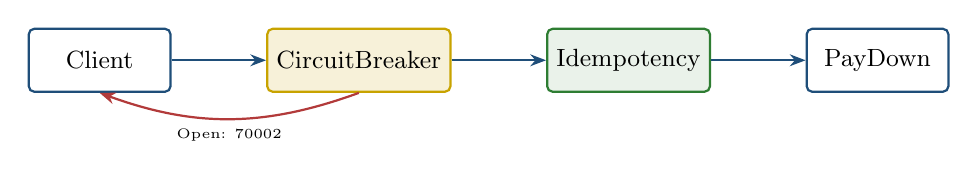
\begin{tikzpicture}[node distance=8mm and 12mm]
  \node[node-box] (cli) {Client};
  \node[node-box,right=of cli,node-warn] (cb)  {CircuitBreaker};
  \node[node-box,right=of cb,node-ok]   (id)  {Idempotency};
  \node[node-box,right=of id] (svc) {PayDown};
  \draw[arrow] (cli) -- (cb);
  \draw[arrow] (cb)  -- (id);
  \draw[arrow] (id)  -- (svc);
  \draw[arrow-bad,bend left=20] (cb.south) to node[below,font=\tiny]{Open: 70002} (cli.south);
\end{tikzpicture}
\vspace{1mm}
\begin{itemize}
  \item 熔断器关心\textbf{保护下游}（5xx 多了断开）。
  \item 幂等关心\textbf{保护用户钱包}（同一笔单只扣一次）。
  \item 两个目标正交，必须\textbf{同时}挂。
  \item 返回 \texttt{200 + status=70002}，HTTP 仍 200 $\to$ app 端老网关不会按 5xx 处理。
\end{itemize}
\srcnote{internal/payment/routes.go:14--21；pkg/e/code.go:58 ErrCircuitOpen=70002}
\end{frame}

\begin{frame}[shrink]{客户端的重试时序（关键业务约定）}
\begin{tikzpicture}[x=1.2mm,y=1mm]
  \node[font=\small] (cli) at (0,0)  {Client};
  \node[font=\small] (svr) at (70,0) {Server};
  \draw[lifeline] (0,-3) -- (0,-58);
  \draw[lifeline] (70,-3) -- (70,-58);
  \draw[arrow]      (0,-10)  -- node[above,font=\tiny]{POST /paydown · IK=abc-001} (70,-10);
  \draw[arrow-bad]  (70,-20) -- node[above,font=\tiny]{70002 (CB Open)} (0,-20);
  \node[font=\tiny] at (35,-30) {等 1s (exp backoff)};
  \draw[arrow]      (0,-40) -- node[above,font=\tiny]{POST /paydown · IK=abc-001 (\textbf{同一个})} (70,-40);
  \draw[arrow]      (70,-52) -- node[above,font=\tiny]{200 success (回放原结果)} (0,-52);
\end{tikzpicture}
\vspace{1mm}
\small \textbf{重试必须带原 Idempotency-Key} —— 万一原请求其实成功（CB 误判 / 网络分区），第二次会被 Idempotency 拦下，返回\textbf{原结果}，绝不二次扣款。这是\textbf{客户端 SDK 必须遵守的契约}，写进对接文档第一页。
\srcnote{middleware/idempotency.go:96--110}
\end{frame}

\begin{frame}[fragile,shrink]{Idempotency 中间件的 responseRecorder}
\begin{lstlisting}[language=Go,firstnumber=17,caption={\srcnote{middleware/idempotency.go:17--31, 96--110}}]
// responseRecorder 拷贝写入的响应体，便于幂等命中时回放
type responseRecorder struct {
    gin.ResponseWriter
    body *bytes.Buffer
}
func (r *responseRecorder) Write(b []byte) (int, error) {
    r.body.Write(b)                        // 旁路缓存
    return r.ResponseWriter.Write(b)       // 同时真写出去
}

// 主流程末尾:
recorder := &responseRecorder{ResponseWriter: c.Writer, body: bytes.NewBuffer(nil)}
c.Writer = recorder
c.Next()
if len(c.Errors) > 0 || recorder.Status() >= http.StatusBadRequest {
    cache.ReleaseIdempotencyLock(c.Request.Context(), key)   // 失败: 回 init
    return
}
cache.CommitIdempotencyResult(c.Request.Context(), key, recorder.body.String())
\end{lstlisting}
\end{frame}

\begin{frame}[shrink]{逐行讲解：responseRecorder 解决了哪个客诉}
\begin{itemize}\small
  \item \textbf{嵌入 gin.ResponseWriter}：包一层而非替换，\texttt{Header/Status/Hijack} 透明转发，链路下游无感。
  \item \textbf{双写}：先写 \texttt{bytes.Buffer} 再调原 \texttt{Writer.Write} —— 顺序很重要，反过来客户端断连时缓存会写不完。
  \item \textbf{失败回滚到 init}：4xx 或 \texttt{c.Errors} $\to$ 同 IK 还能再试（业务失败 $\neq$ 永久失败）—— 对应客诉"我密码输错了重输一次不行"的合理诉求。
  \item \textbf{成功提交到 done}：把完整 JSON 写进 Redis done 态 $\to$ 后续同 IK 由 Lua 直接回放，\textbf{业务代码不再执行}—— 这是"重复扣款"客诉归零的关键。
\end{itemize}
\srcnote{middleware/idempotency.go:17--112}
\end{frame}

\begin{frame}[shrink]{Lua 脚本里的四态机 + 业务码 + 客服话术}
\resizebox{0.85\textwidth}{!}{%
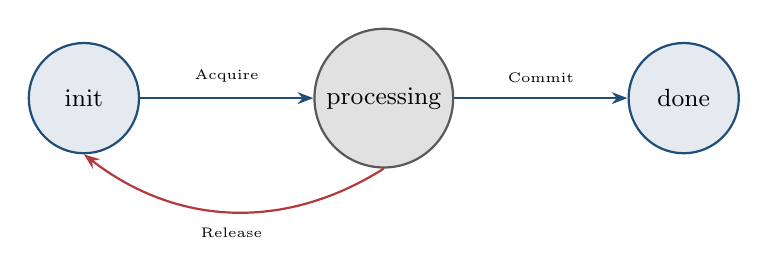
\begin{tikzpicture}[node distance=10mm and 22mm,font=\scriptsize]
  \node[node-state,node-state-normal] (init) {init};
  \node[node-state,node-state-transition,right=of init] (proc) {processing};
  \node[node-state,node-state-normal,right=of proc] (done) {done};
  \draw[arrow] (init) -- node[above=2pt,pos=0.5,font=\tiny]{Acquire} (proc);
  \draw[arrow] (proc) -- node[above=2pt,pos=0.5,font=\tiny]{Commit} (done);
  \draw[arrow-bad] (proc.south) to[bend left=35] node[below=2pt,pos=0.5,font=\tiny]{Release} (init.south);
\end{tikzpicture}}
\vspace{1mm}
\begin{tabular}{@{}llll@{}}
\toprule
状态码 & 含义               & 客户端动作          & 客服话术       \\
\midrule
30001  & token 错误         & 重登录              & "请重新登录" \\
60001  & IK 不存在/过期    & 重新申领            & "刷新页面再试" \\
60002  & 幂等命中处理中    & 等 1s 再试          & "正在处理，请稍候" \\
70001  & 限流              & 退避重试            & "请求过频，稍后再试" \\
70002  & 熔断 Open         & 指数退避 + 带原 IK  & "支付通道维护中" \\
\bottomrule
\end{tabular}
\srcnote{repository/cache/idempotency.go:32--50；pkg/e/code.go:35--58}
\end{frame}

\begin{frame}[shrink]{客服话术帧：用户报"扣了钱订单还显示未支付"}
\small
\begin{tabular}{@{}lp{8cm}@{}}
\toprule
表征 & 排查路径 \\
\midrule
DB 余额已减 + order=UnPaid & \textbf{不可能}，TX 原子。让用户清缓存刷新 \\
DB 余额未减 + order=UnPaid & 真的没扣，让用户重试 \\
DB 余额已减 + order=PendingShipping + 前端显示 UnPaid & 前端缓存问题，让用户下拉刷新；底层正常 \\
返回 60002 & 让用户等 1 秒；上一次请求仍在处理 \\
返回 70002 & 通道维护中，30s 后重试；自动发 5 元补偿券 \\
返回 30001 & token 过期，让用户重新登录后原 OrderId 仍可付 \\
\bottomrule
\end{tabular}
\vspace{1mm}
\keypoint{客服\textbf{不查代码}，只查\textbf{业务码 + DB 状态}两件事就能判断 90\% 的支付客诉。这是业务码表存在的根本意义。}
\srcnote{pkg/e/code.go:35--58；internal/payment/service.go:53--186}
\end{frame}

% ============================================================
\section{失败兜底、SLO 与压测数字}
% ============================================================

\begin{frame}[shrink]{支付失败链路 —— Saga 回滚}
\begin{tikzpicture}[node distance=6mm and 9mm]
  \node[node-box] (p1) {/paydown\\TX fail};
  \node[node-box,right=of p1] (p2) {Order=UnPaid};
  \node[node-box,right=of p2,node-warn] (p3) {30min\\等支付};
  \node[node-box,below=of p3,node-bad] (p4) {Cron 扫\\超时未付};
  \node[node-box,left=of p4] (p5) {Saga 关单\\+ 释放预占};
  \node[node-box,left=of p5] (p6) {outbox\\order.cancelled};
  \draw[arrow] (p1) -- (p2);
  \draw[arrow] (p2) -- (p3);
  \draw[arrow-alert] (p3) -- (p4);
  \draw[arrow] (p4) -- (p5);
  \draw[arrow] (p5) -- (p6);
\end{tikzpicture}
\vspace{1mm}
\begin{itemize}
  \item 支付失败 = TX 回滚 = \texttt{order.Type} 仍 UnPaid，库存\textbf{从未真扣}。
  \item 30min 未续支付 $\to$ Cron + RMQ 双保险（deck 09）$\to$ \texttt{CancelUnpaidOrder}。
  \item Saga 不回写 \texttt{product.Num}（从未扣过），仅释放 Redis \texttt{reserved}；满减预算退还由 promo 侧消费 \texttt{order.cancelled} 事件异步完成。
\end{itemize}
\srcnote{internal/order/cancel.go:19--68；deck 09 关单衔接}
\end{frame}

\begin{frame}[fragile,shrink]{CancelUnpaidOrder 的幂等设计}
\begin{lstlisting}[language=Go,firstnumber=31,
  caption={\srcnote{internal/order/cancel.go:31--53}}]
err = baseDao.DB.Transaction(func(tx *gorm.DB) error {
    ok, err := NewOrderDaoByDB(tx).CloseOrderWithCheck(orderNum)
    if err != nil { return err }
    if !ok { return nil }                  // 已被别处关过, no-op
    closed = true
    return outbox.NewOutboxDaoByDB(tx).Insert(
        "order", "OrderCancelled", "order.cancelled", order.ID,
        events.OrderCancelled{
            OrderID: order.ID, OrderNum: orderNum,
            UserID: order.UserID, ProductID: order.ProductID,
            Num: order.Num, Reason: "timeout",
            PromoRuleID:        order.PromoRuleID,        // 满减自包含
            PromoDiscountCents: order.PromoDiscountCents, // 预算异步退还
        },
    )
})
\end{lstlisting}
\vspace{1mm}
\small \textbf{CloseOrderWithCheck} 用 \texttt{WHERE type=待付款} 条件 update，第二次调用自然 affected=0 $\to$ 函数变 no-op。这是\textbf{用 DB 行做幂等键}。Redis 释放走 TX 外，失败仅记日志，对账兜底；满减预算退还\textbf{不在关单事务里同步做} —— 事件载荷自带 \texttt{promo\_rule\_id / promo\_discount\_cents}，promo 侧消费 \texttt{order.cancelled} 异步退还（幂等台账，OrderID 唯一索引）。业务承诺：\textbf{用户 / 客服 / Cron / RMQ 四个调用方都能反复点关单，库存绝不漏放}。
\end{frame}

\begin{frame}[shrink]{满减实付口径：为什么不能用折前价计费 / 退款}
\begin{itemize}\small
  \item 一个满减订单：商品 \texttt{Money*Num = 100} 元，命中"满 80 减 20"，用户\textbf{实际只付 80}（\texttt{FinalCents = 80}）。
  \item \textbf{扣款若用折前价 100}：买家被多扣 20 元 —— 满减优惠被吞掉，直接客诉 + 平台信任受损（"明明满减了还按原价扣"）。
  \item \textbf{退款若用折前价 100}：用户只付了 80，却退回 100 —— 平台\textbf{超额退款 20 元资损}。更糟的是满减预算已随 \texttt{order.refunded} 事件由 promo 侧退还，钱包再按原价退 = \textbf{双重退还}。
  \item 统一解法：payment 扣款与 refund 退款\textbf{都取折后实付 \texttt{FinalCents}}，只有 \texttt{FinalCents} 未写入（老订单 / 老客户端没读这字段）时才回退 \texttt{Money*Num} 兜底。
\end{itemize}
\keypoint{满减订单的"应收 / 应退"金额\textbf{只有一个口径}：用户实付 \texttt{FinalCents}。计费用折前价多扣买家，退款用折前价超退资损 —— 两头都是钱，必须统一。}
\srcnote{internal/payment/service.go:79--82 payable 口径；internal/refund/service.go:106--112 退款口径}
\end{frame}

\begin{frame}[fragile,shrink]{退款侧的实付口径（与支付侧对齐）}
\begin{lstlisting}[language=Go,firstnumber=106,
  caption={\srcnote{internal/refund/service.go:106--112}}]
// 退款额取实付口径，与 payment 侧保持一致：命中满减以折后实付 FinalCents 为准，
// 仅当 FinalCents 未写入（<=0）时回退到折前价 Money*Num。
// 用折前价会把满减优惠重复退还（promo 已随事件退预算，钱包再按原价退即双重退还）
amount := order.FinalCents
if amount <= 0 {
    amount = order.Money * int64(order.Num)
}
\end{lstlisting}
\vspace{1mm}
\small 退款侧的回退判据是 \texttt{FinalCents <= 0}（未写入才回退），与支付侧用 \texttt{PromoRuleID != 0}（命中即取折后价）略有差异：退款拿到的是已落库订单，\texttt{FinalCents} 一定已写定，\texttt{<= 0} 只为兼容历史脏数据。\texttt{amount} 随 \texttt{order.refunded} 事件下发，下游 wallet 服务据此退款；满减预算退还由 promo 侧消费同一事件\textbf{异步}完成（事件自带 \texttt{promo\_rule\_id / promo\_discount\_cents}），两者各退各的、不重不漏。
\srcnote{internal/refund/service.go:109--132 事件载荷；internal/order/model.go:30--34 FinalCents 注释}
\end{frame}

\begin{frame}[shrink]{支付链路 SLO 承诺}
\small
\begin{tabular}{@{}llll@{}}
\toprule
指标 & 承诺值 & 实测对照 & 兜底机制 \\
\midrule
可用率 & 99.95\% & 全链 idempotency 50K RPS 0\% err & CB + outbox + Saga \\
p99 延迟 & < 500 ms & p95 2.33 ms（idempotent replay） & responseRecorder cache \\
重复扣款率 & 0 & 755K req $\to$ 1 DB row & Lua done 态回放 \\
扣款不出货 & 0 & outbox 与 TX 原子 & deck 11 outbox 主题 \\
P0 不挂限流 & ✓ & /paydown 路由仅挂 CB + Idem & 不挂 TokenBucket/SW \\
\bottomrule
\end{tabular}
\vspace{2mm}
\small "P0 不挂限流"是\textbf{业务承诺}：宁可下游慢、不能上游 429。下单 / 支付靠缓存 + 异步削峰扛峰值（deck 10）。
\srcnote{README.md §业务承诺；stressTest/REPORT.md §1 + §4}
\end{frame}

\begin{frame}[shrink]{基线对照：两个中间件接入后的吞吐}
\begin{tabular}{@{}lrr@{}}
\toprule
链路 & RPS & p95 \\
\midrule
/ping 基线 (无中间件)                & 64{,}254 & 3.51 ms \\
/product/show (无 CB / 无 Idem)      & 62{,}226 & 3.01 ms \\
/orders/create (\textbf{Idempotency}) & 50{,}319 & 2.33 ms \\
/skill\_product/skill (RateLimit)    & 52{,}082 & 1.24 ms \\
\bottomrule
\end{tabular}
\vspace{2mm}
\begin{itemize}
  \item Idempotency 让吞吐 62K $\to$ 50K，约 \textbf{19\% 损耗}。换来"755K 请求 $\to$ 1 笔订单"的强幂等。
  \item 业务侧的取舍：\textbf{19\% 吞吐 vs 0 起重复扣款客诉}，毫无悬念选后者。
  \item CircuitBreaker Closed 态\textbf{零锁开销}（仅 atomic.Load），吞吐影响可忽略。
\end{itemize}
\srcnote{stressTest/REPORT.md §1 链路压测表前 7 行}
\end{frame}

\begin{frame}[shrink]{Idempotency 的极限场景：755K 请求 $\to$ 1 笔订单}
\begin{itemize}
  \item 50 VU $\times$ 15s 用\textbf{同一个 IK} 反复打 \texttt{/orders/create}。
  \item 累计 \textbf{755{,}033 次请求}，DB 实际订单数 \textbf{= 1}：
  \begin{itemize}
    \item \texttt{SELECT COUNT(*) FROM `order` WHERE user\_id=10 AND created\_at > NOW() - 2 MIN} $\to$ 1
  \end{itemize}
  \item 第一次走完业务后，后续全部由 Lua 读 \texttt{done} 态直接回放 $\to$ 50K RPS。
  \item \textbf{业务承诺}：客户端在熔断反复触发期间无脑重试 10K 次，仍只扣一次款 —— 这是写进 SDK 文档的合同。
\end{itemize}
\keypoint{压测数字背后是合同：\textbf{重复扣款率 = 0}。客服 / 财务 / 风控都靠这个承诺生存。}
\srcnote{stressTest/REPORT.md §4 幂等中间件压测}
\end{frame}

\begin{frame}[shrink]{把 paydown 的设计翻译成业务承诺}
\begin{tabular}{@{}ll@{}}
\toprule
技术选择                  & 业务承诺                            \\
\midrule
AES-128-CBC + 双密钥      & DBA 拿 dump 也看不到余额            \\
6 位支付密码不存盘        & 整库泄漏没密码也解不开              \\
单次 TX 多件事原子        & 不会出现"扣了钱没改订单"            \\
debit/credit 流水同事务   & 余额必有流水，全表借贷恒等，可对账   \\
实付取 FinalCents         & 满减不多扣买家、退款不超退资损       \\
outbox 在 TX 内写         & 不会出现"扣了钱下游没收到"          \\
CircuitBreaker 5/10s/3   & 第三方挂了 5\% 用户受影响，不是 100\% \\
Idempotency 全程伴随     & 重试 10K 次也只扣一次               \\
Saga 30min 关单           & 用户忘付款，库存自动释放              \\
业务码 60002/70002/30001  & 客服查码即可定位 90\% 客诉            \\
\bottomrule
\end{tabular}
\vspace{1mm}
\small 八条产品 / 运营 / 客服三方都能背的话术，每条都在代码里找得到位置。
\srcnote{internal/payment/routes.go:14--21 + internal/payment/service.go:35--201}
\end{frame}

\begin{frame}[shrink]{业务边界回顾：本支付\textbf{不做}什么（再次诚实）}
\begin{itemize}
  \item \textbf{不真接支付宝 / 微信 / 银联} —— 路线图 step 1
  \item \textbf{不做实名 KYC} —— 持牌支付公司的事
  \item \textbf{不做风控引擎} —— 路线图 step 2
  \item \textbf{不做反洗钱} —— 独立合规系统
  \item \textbf{不做商家分账} —— 路线图 step 3
  \item \textbf{不做发票管理} —— 财税系统
  \item \textbf{未做清单完整版}：\texttt{docs/architecture/feature-matrix.md}
\end{itemize}
\keypoint{诚实划边界给商家 / 合规一个交代，比"全堆 feature"更可信。MVP 阶段把\textbf{扣款 + 入账 + 状态机推进 + 防重}做到工业级。}
\srcnote{README.md §业务边界；docs/architecture/feature-matrix.md}
\end{frame}

% ============================================================
\appendix
% ============================================================

\begin{frame}[shrink]{Q\&A（上）—— 业务侧高频问题}
\small
\textbf{Q1}：为什么金额不直接 \texttt{decimal} 存，非要 AES？\\
\hspace{4mm} A：合规审计要求"敏感金额字段不得明文落盘"。AES + 服务端密钥 + 用户密码双因子，DBA 拿 dump 也解不开。代价是 SQL 不能 \texttt{SUM}，业务侧用结算服务批跑兜底。

\vspace{1mm}
\textbf{Q2}：为什么不接真实支付宝？\\
\hspace{4mm} A：MVP 阶段聚焦交易闭环，第三方对接由 wallet 服务消费 outbox 完成（路线图）。\textbf{熔断器 + 幂等 + outbox 已就位}，接入只换 Gateway 实现，不改架构。

\vspace{1mm}
\textbf{Q3}：熔断打开期间用户体验怎么办？\\
\hspace{4mm} A：(1) 立即返回 70002 + 客服话术（"通道维护中，30s 后重试"）；(2) 自动发 5 元补偿券回赠；(3) 监控触发 oncall + 客服群通知。运营 SOP 写在 §4。

\vspace{1mm}
\textbf{Q4}：为什么支付密码不存数据库？\\
\hspace{4mm} A：用户每次手输，整库 dump 也解不开。代价 = 用户每次支付要手输；收益 = 任何拖库事件都不会暴露余额。客服重置走"核身 + 余额冻结 48h"流程。
\end{frame}

\begin{frame}[shrink]{Q\&A（下）—— 技术侧追问}
\small
\textbf{Q5}：支付密码输错了，用户会看到什么？\\
\hspace{4mm} A：\texttt{DecryptMoney} 把"错误密钥去填充 panic / 解出乱码"统一折叠为 \texttt{ErrMoneyKeyIncorrect}（支付密码错误），TX 回滚不扣款。早期实现这条路径会 panic 带崩整个请求；穷举防护交给限流 + 熔断 + 幂等三层，不靠含混报错。

\vspace{1mm}
\textbf{Q6}：为何不用 Redis 分布式锁做幂等，要用 Lua？\\
\hspace{4mm} A：分布式锁只解决"不重入"，不解决"结果回放"。Lua 是真状态机 (init/processing/done)：第一次走完后，同 IK 请求直接 Lua 内回放，\textbf{不进业务代码}。

\vspace{1mm}
\textbf{Q7}：CircuitBreaker 阈值 5 / 10s / 3 怎么调的？\\
\hspace{4mm} A：5 = 防误熔（1-2 次抖动不算）；10s = 第三方重启中位数；3 = HalfOpen 探测样本够。当前硬编码，路线图改成 env 配置 + 按时段动态调整。

\vspace{1mm}
\textbf{Q8}：支付链路怎么保证 P0 不挂限流？\\
\hspace{4mm} A：\texttt{/paydown} 路由\textbf{只挂 CB + Idem}，不挂 TokenBucket / SlidingWindow。上游靠下单 + 缓存削峰，下游靠熔断保护 —— 宁可下游慢、不能上游 429。
\end{frame}

\begin{frame}[shrink]{代码位置一览}
\scriptsize
\begin{description}
  \item[PayDown 主体]\srcnote{internal/payment/service.go:38--234}
  \item[资金台账 / 复式记账]\srcnote{internal/money/ledger\_model.go:7--36；internal/money/ledger\_repo.go:20--38}
  \item[实付口径 FinalCents]\srcnote{internal/payment/service.go:79--82；internal/refund/service.go:106--112}
  \item[台账 AutoMigrate 注册]\srcnote{internal/migrate/migrate.go:44}
  \item[AES 加解密]\srcnote{internal/user/model.go:64--101；pkg/utils/encryption/money\_encrypt.go}
  \item[CircuitBreaker]\srcnote{middleware/circuitbreaker.go:17--136}
  \item[Idempotency]\srcnote{middleware/idempotency.go:17--112；repository/cache/idempotency.go:32--90}
  \item[paydown 路由 + 中间件栈]\srcnote{internal/payment/routes.go:12--28}
  \item[支付失败 Saga]\srcnote{internal/order/cancel.go:19--68}
  \item[业务码表]\srcnote{pkg/e/code.go:35--58；pkg/e/msg.go:48--52}
  \item[压测数字]\srcnote{stressTest/REPORT.md §1 链路压测、§4 幂等中间件}
  \item[业务边界 / SLO]\srcnote{README.md §业务承诺、§业务边界、§典型用户旅程}
\end{description}
\keypoint{配套：deck 01（鉴权 / 双 token） / deck 04（下单 + outbox） / deck 09（关单 + 状态机） / deck 11（一致性主题）。}
\end{frame}

\end{document}
